\documentclass[aspectratio=169]{beamer}
%\usecolortheme{beaver}
\usepackage[english,ukrainian]{babel}
\usepackage{hyperref}
\hypersetup{colorlinks,urlcolor=blue}
\makeatletter
\DeclareUrlCommand\ULurl@@{%
  \def\UrlFont{\ttfamily\color{blue}}%
  \def\UrlLeft{\uline\bgroup}%
  \def\UrlRight{\egroup}}
\def\ULurl@#1{\hyper@linkurl{\ULurl@@{#1}}{#1}}
\DeclareRobustCommand*\ULurl{\hyper@normalise\ULurl@}
\makeatother
\usepackage[table]{colortbl}
\usecolortheme{whale}
\usepackage{etoolbox,refcount}
\usepackage{multicol}

\newcounter{countitems}
\newcounter{nextitemizecount}
\newcommand{\setupcountitems}{%
  \stepcounter{nextitemizecount}%
  \setcounter{countitems}{0}%
  \preto\item{\stepcounter{countitems}}%
}
\makeatletter
\newcommand{\computecountitems}{%
  \edef\@currentlabel{\number\c@countitems}%
  \label{countitems@\number\numexpr\value{nextitemizecount}-1\relax}%
}
\newcommand{\nextitemizecount}{%
  \getrefnumber{countitems@\number\c@nextitemizecount}%
}
\newcommand{\previtemizecount}{%
  \getrefnumber{countitems@\number\numexpr\value{nextitemizecount}-1\relax}%
}
\makeatother    
\newenvironment{AutoMultiColItemize}{%
\ifnumcomp{\nextitemizecount}{>}{3}{\begin{multicols}{2}}{}%
\setupcountitems\begin{itemize}}%
{\end{itemize}%
\unskip\computecountitems\ifnumcomp{\previtemizecount}{>}{3}{\end{multicols}}{}}
\usepackage[utf8]{inputenc}

\title{Формування дивідендної політики корпорації (на прикладі компаній, що входять до індексу Standard \& Poor's 100)}
\author{Студент 2 курсу магістратури\\спеціальності 072 «Фінанси, банківська справа та страхування»\\ОП «Корпоративні фінанси» Тараба В. С.\\ Науковий керівник: д. е. н., доцент Любкіна О. В.}
\institute{Київський національний університет імені Тараса Шевченка\\Економічний факультет\\Кафедра фінансів}

\begin{document}
	
\begin{frame}
\titlepage
\end{frame}

\begin{frame}
\frametitle{План презентації}
\setbeamertemplate{section in toc}[circle]
%\setbeamercolor{section in toc}{fg=UniBlue}
%\setbeamercolor*{section in toc}{fg=UniBlue}
\tableofcontents
\end{frame}

\section{Опис дослідження}

\begin{frame}
\frametitle{Опис дослідження}
\begin{itemize}
\item \alert {Метою дослідження} є визначення видів дивідендної політики на основі даних для компаній, що входять до індексу S&P 100.
\tinyskip
\item \alert {Об’єктом дослідження} є компанії, що входять до індексу S&P 100.
\tinyskip
\item \alert {Предметом дослідження} є види дивідендної політики та їх практична реалізація.
\tinyskip
\item \alert {Завданнями дослідження} є:
\begin{itemize}
    \item[\textcolor{orange}{\textbullet}] розглянути теоретичні засади формування дивідендної політики (основні чинники, що впливають на формування дивідендної політики компаній, види дивідендної політики та їх особливості); 
    \item[\textcolor{orange}{\textbullet}] розглянути можливості для автоматизації процесу збору та обробки та даних та обрати оптимальний варіант; 
    \item[\textcolor{orange}{\textbullet}] сформувати критерії для визначення видів дивідендної політики на основі даних;
    \item[\textcolor{orange}{\textbullet}] виконати збір даних за останні 10 років (2014-2023 рр), які необхідні для визначення виду дивідендної політики;
    \item[\textcolor{orange}{\textbullet}] визначити види дивідендної політики компаній, що входять до індексу S\&P 100
\end{itemize}
\end{itemize}
\end{frame}


\section{Ключові фінансові індикатори видів дивідендної політики}
\begin{frame}
\frametitle{Ключові фінансові індикатори видів дивідендної політики}

\end{frame}

\begin{frame}
\frametitle{Види дивідендної політики}

\end{frame}

\section{Збір та підготовка даних (формування бази даних)}
\begin{frame}
\begin{itemize}
\item Для збору, обробки даних,та розрахунків використовувалися python, SQL, Power BI.
\bigskip
\item \alert {Процес збору і обробки даних} складається з 4 основних етапів.
\begin{itemize}
    \item[\textcolor{orange}{\textbullet}] отримання списку тікерів, що входять до S&P 100 та загальної інформації для кожного тікеру (назва компанії, галузь тощо);
    \item[\textcolor{orange}{\textbullet}] збір по показниках DPS (дивіденди на одну звичайну акцію), EPS (чистий прибуток на одну звичайну акцію);
    \item[\textcolor{orange}{\textbullet}] приведення до єдиного формату та звірка показників, отриманих з різних джерел, для гарантування якості даних;
    \item[\textcolor{orange}{\textbullet}] розрахунок DPR (коефіцієнт виплати дивідендів) та побудова Power BI звіту на основі зібраних даних для визначення видів дивідендної політики та аналізу отриманих результатів.
\end{itemize}
\bigskip
\item \alert {Основними джерелами даних} є сайти finance.yahoo.com, stockanalysis.com, macrotrends.com, nasdaq.com; додаткові джерела даних:* sec.gov, investing.com, morningstar.com та сайти компаній.
\end{itemize}
\bigskip
\scriptsize \textcolor{gray}{* використовувалися лише за потреба в окремих випадках} 
\frametitle{Збір та підготовка даних (формування бази даних)}

\end{frame}

\begin{frame}
\frametitle{Формування бази даних (спрощена версія)}
\begin{center}
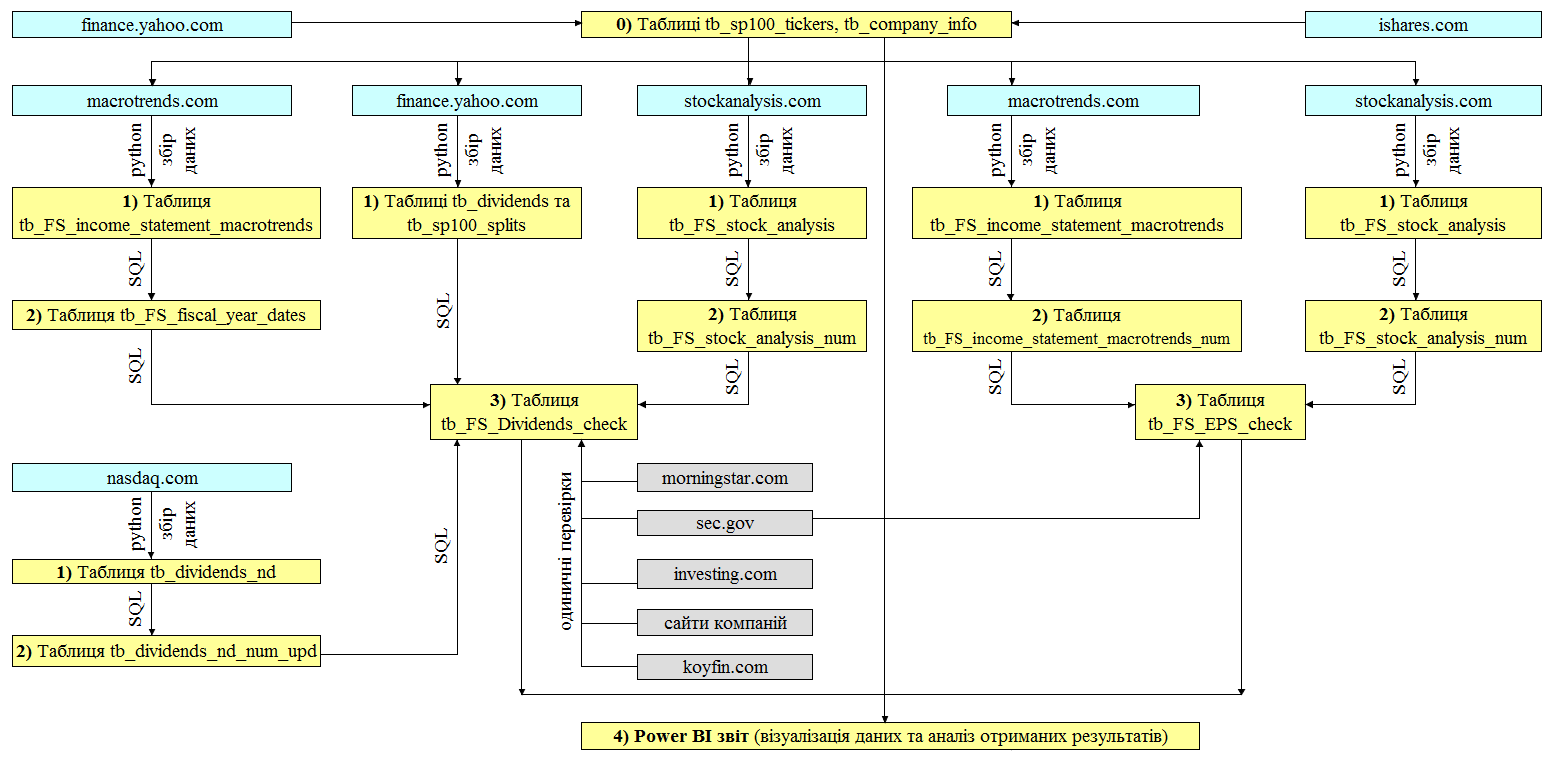
\includegraphics[scale=0.35]{Data Flow full.png}
\end{center}
\end{frame}

\section{Ідентифікація виду дивідендної політики компаній, що входять до індексу Standard \& Poor's 100}
\begin{frame}
\frametitle{Ідентифікація видів дивідендної політики компаній, що входять до індексу Standard \& Poor's 100}

\end{frame}

\begin{frame}
\frametitle{Дані - Індекс  українських  акцій}
\begin{center}
\begin{itemize}
\item \alert {Індекс  українських  акцій}  (Ukrainian  Equities  Index,  UX  Index) - розраховується ПАТ «Українська біржа» починаючи з 26 березня 2009 року.
\smallskip
\item  \alert {Період:} з 2009 року по 25 лютого 2022 року (остання доступна дата, після цієї дати 
торги  зупинено)
\end{itemize}
\tinyskip
\includegraphics[scale=0.5]{Index.png}
\tinyskip
\end{center}
\scriptsize \textcolor{gray}{* З  початком  російського  вторгнення  торги  на  біржі було  припинено.} 
\end{frame}

\section{Висновки}

\begin{frame}
\frametitle{Висновки}
\begin{itemize}
\item Усі побудовані торгові стратегії, незалежно від того, чи базувалися вони на 
сигналах  методів  технічного  аналізу,  чи  на  прогнозах  моделей  машинного навчання, \alert {\textbf{виявилися збитковими}}; результати наших торгових стратегій програють в порівнянні з пасивною  стратегією  buy-and-hold.  
\bigskip
\item Цей  результат  узгоджується  з  теорією ефективних ринків, яка виключає можливість прибутковості технічного аналізу зокрема та активних інвестиційних стратегій в цілому.
\bigskip
\item Отже, ані використання методів технічного аналізу, ані використання методів машинного навчання \alert {\textbf{не дозволило б нам переграти ринок}} (для індексу українських акцій UX за період з 2008 по 2022 роки)
\bigskip
\definecolor{cadmiumgreen}{rgb}{0.0, 0.42, 0.24}
\item \textcolor{blue} {У подальшому доцільно було б розглянути} інші  методи  машинного навчання, збільшити кількість індексів, та спробувати замінити сигнали  методів технічного  аналізу  фундаментальними даними
\bigskip
\end{itemize}
\end{frame}

\section{Q\&A}

\begin{frame}
\frametitle{Q\&A}
\begin{center}
\bigskip
\textcolor{blue}{\huge Дякую за увагу!} \\
\end{center}
\begin{multicols}{2}

\vbox{\vspace{0.8cm}}
Дані та код для обробки даних, навчання моделей, розрахунків та побудови графіків (.ipynb), а також .pbix файли доступні в репозиторії (github), перейти до якого можна {відсканувавши QR-код праворуч.}
\columnbreak
\hspace{5mm}
\includegraphics[scale=0.12]{qr-code.png}
\end{multicols}
\end{frame}

\begin{frame}
\frametitle {Q\&A - Формування дивідендної політики корпорації (на прикладі компаній, що входять до індексу Standard \& Poor's 100 }
\setbeamertemplate{section in toc}[circle]
%\setbeamercolor{section in toc}{fg=UniBlue}
%\setbeamercolor*{section in toc}{fg=UniBlue}
\tableofcontents
\end{frame}

\end{document}